\section{Methodology}

\section{Data and Processing Overview}

\subsection{Data}

Comparing the performance and features of gene finding tools, both
qualitative and quantitative, in the context of any set of genomes is
important for those interested in selecting a specific gene finding
tool. To accent(?) the processing for genomes of interest, those being
DC1 and Tsht20, we should include other previously assembled
\textit{Trichoderma} assemblies. Currently selected genomes include
\textit{Trichoderma reesei}, \textit{Trichoderma harzianum}, and
\textit{Trichoderma virens}, with \textit{Trichoderma reesei} being
the 'reference' in this case, as it is well studied and there are
several patents involving it's use a organsim for production of
compounds such as antibiotics in industrial applications.

The general methodology for this work is described in figure 1. Each
portion of this figure is discussed in detail in this section.

\begin{figure}
  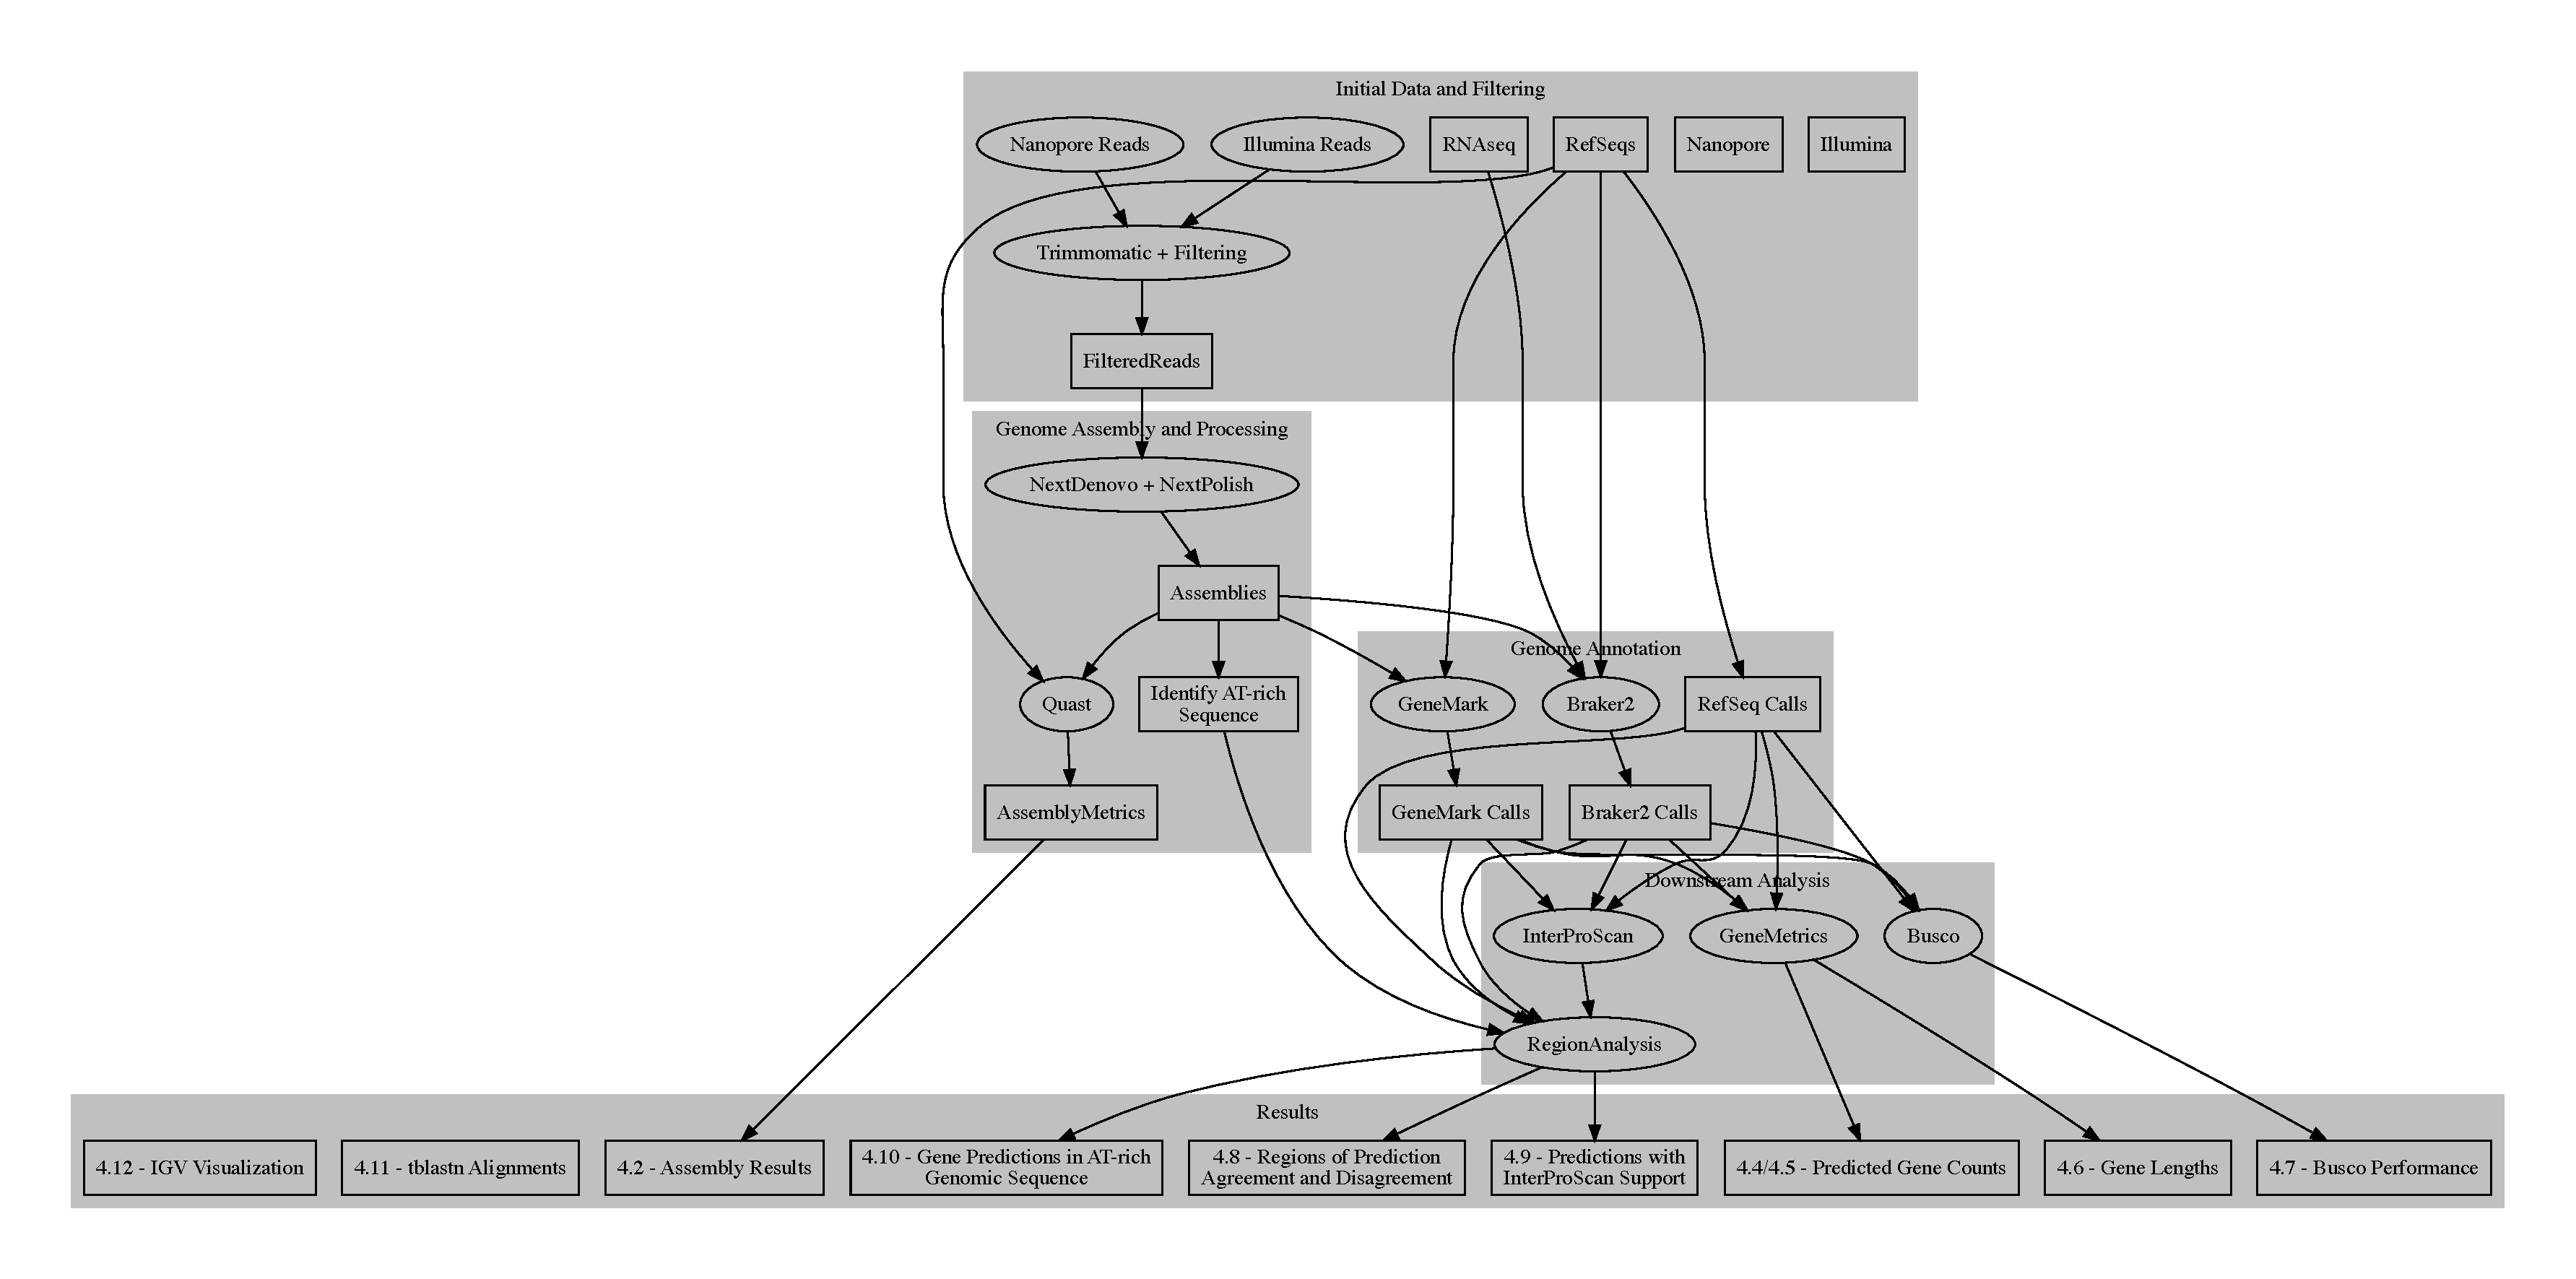
\includegraphics[width=\textwidth]{./figures/data-flowchart.pdf}
  \caption{A flowchart of the methodology followed for this research. Sections are separated based the general process they are associated with (i.e. input data, assembly, gene finding and downstream analysis).}
\end{figure}

\section{Assembly and Annotation}

In an attempt to produce high quality assemblies of DC1 and Tsth20, We
decided on a set of tools named NextDenovo and NextPolish as they have
produced excellent assemblies based on previous experience. (should
find a citation to confirm this)

(Might be better for discussion or omitted since it is specific to our
setup) Initial attempts to run the example dataset resulted in
permissions errors due to the management of the storage system being
used, which were encountered with other tools in the past. To remedy
this, the software installation was copied to RSMI's scratch space on
Copernicus. Once the approriate permissions were given to run
nextDenovo, the example dataset was run without issue.

Following assembly using nextDenovo, Illumina sequence data from DC1
and Tsth20 was used to polish each respective genome using
nextPolish. Default parameters were used from assembly except for
modification of the parallel option to reduce processing times.

\subsection{Repeat Masking}

In order to evaluate the performance of gene finding tools in
repetitive or low complexity regions in the context of
\textit{Trichoderma} genomes, we must first identify said regions in
the genomes considered. To do this, the GenericRepeatFinder tool was
used, which is a \textit{de novo} repeat detection tool
\cite{10.1104/pp.19.00386}. GenerifRepeatFinder detects three
different types of repeats, those being MITEs, TDRs and TIRs. Commands
used for this program follow the example commands provided on the
GitHub page for the GenericRepeatFinder project.

\subsection{GeneMark-ES}

To begin, GeneMark-ES was run as it requires no prior information or
alignments in order to run. In this case GeneMark-ES has an option
specifically for fungal genomes, which was used in this case. Apart
from the fungal option, the only additional options supplied were for
output format of GFF3 and number of cores for reduced processing time.

General command structure for GeneMark-ES:

gmes\_petap.pl --ES --fungus
--format gff3 --cores 48 --sequence /path/to/sequence

\subsection{Braker2}

As mentioned previously, \textit{Trichoderma reesei} was selected as
the \'reference\' genome for this work. With this in mind, several
short read archives (SRAs) from \textit{T. reesei} were selected for
Augustus training. Following Augustus training, the model for
\textit{T reesei} was applied to all genomes considered. Settings and
procedures from running Braker2 are described below.

The variables that need to be set are AUGUSTUS\_CONFIG\_PATH and
TSEBRA\_PATH. Augustus, by defuault, tries to write species
information to the location where the software is installed. In this
case, we don'thave write permissions to the compute canada software
stack hosted byt Research Computing, so the AUGUSTUS\_CONFIG\_PATH
variable must be set in order to create a writeable directory. As long
as that path has a directory within it called braker, and a species
directory within the braker directory, things should go
smoothly. TSEBRA is a set of scripts also made by the creators of
Braker and is required to merge results from the various gene
prediction tools involved in the Braker2 pipeline. The TSEBRA\_PATH
simply points to the directory where TSEBRA is located Both Braker2
and TSEBRA can be cloned directly from GitHub (links to come)

\section{Identification of Overlapping Features and Regions}

Feature Identification: To first undertand how gene prediction tools
perform in comparison to other gene prediction tools, we must identify
features. This identification of features will help us descirbe the
similarities, and differences between gene finding tools. A feature,
in this context, is any feature stated within a Genomic Feature Format
file (GFF) provided to the program, in which mutliple GFF files can be
provided. The definition of a feature, for this application, is an
object that contains a contig ID, a start position, an end position
and a strand property. In the context of features on different
strands, start and stop positions of features are sorted based on left
and right positions of the feature in respect to the reference
sequence.

Region Identification: In addition to feature creation, we will also
identify regions of overlapping features based on the precitions from
each gene finding tool. These regions will help identify the
agreements, or disagreements, between different gene-finding tools. A
region, in this context, is a set of overlapping features, all of
which overlap at least one other feature in the region. With each
overlap, there will be an overlap type. These types can be defined
based on Allen's Interval Calculus (reference), with the exception of
features that start beyond the end point of the current region.


=======
Example command for braker2:

/scratch/p2irc/p2irc\_rsmi/cbe453/masters/software/braker2/BRAKER/scripts/braker.pl
--gff3 --threads 60
--TSEBRA\_PATH=/scratch/p2irc/p2irc\_rsmi/cbe453/masters/software/braker2/tsebra/TSEBRA/bin/
--genome /path/to/sequence --species=TreeseiFungal --fungus
--useexisting
